
% Default to the notebook output style

    


% Inherit from the specified cell style.




    
\documentclass[11pt]{article}

    
    
    \usepackage[T1]{fontenc}
    % Nicer default font (+ math font) than Computer Modern for most use cases
    \usepackage{mathpazo}

    % Basic figure setup, for now with no caption control since it's done
    % automatically by Pandoc (which extracts ![](path) syntax from Markdown).
    \usepackage{graphicx}
    % We will generate all images so they have a width \maxwidth. This means
    % that they will get their normal width if they fit onto the page, but
    % are scaled down if they would overflow the margins.
    \makeatletter
    \def\maxwidth{\ifdim\Gin@nat@width>\linewidth\linewidth
    \else\Gin@nat@width\fi}
    \makeatother
    \let\Oldincludegraphics\includegraphics
    % Set max figure width to be 80% of text width, for now hardcoded.
    \renewcommand{\includegraphics}[1]{\Oldincludegraphics[width=.8\maxwidth]{#1}}
    % Ensure that by default, figures have no caption (until we provide a
    % proper Figure object with a Caption API and a way to capture that
    % in the conversion process - todo).
    \usepackage{caption}
    \DeclareCaptionLabelFormat{nolabel}{}
    \captionsetup{labelformat=nolabel}

    \usepackage{adjustbox} % Used to constrain images to a maximum size 
    \usepackage{xcolor} % Allow colors to be defined
    \usepackage{enumerate} % Needed for markdown enumerations to work
    \usepackage{geometry} % Used to adjust the document margins
    \usepackage{amsmath} % Equations
    \usepackage{amssymb} % Equations
    \usepackage{textcomp} % defines textquotesingle
    % Hack from http://tex.stackexchange.com/a/47451/13684:
    \AtBeginDocument{%
        \def\PYZsq{\textquotesingle}% Upright quotes in Pygmentized code
    }
    \usepackage{upquote} % Upright quotes for verbatim code
    \usepackage{eurosym} % defines \euro
    \usepackage[mathletters]{ucs} % Extended unicode (utf-8) support
    \usepackage[utf8x]{inputenc} % Allow utf-8 characters in the tex document
    \usepackage{fancyvrb} % verbatim replacement that allows latex
    \usepackage{grffile} % extends the file name processing of package graphics 
                         % to support a larger range 
    % The hyperref package gives us a pdf with properly built
    % internal navigation ('pdf bookmarks' for the table of contents,
    % internal cross-reference links, web links for URLs, etc.)
    \usepackage{hyperref}
    \usepackage{longtable} % longtable support required by pandoc >1.10
    \usepackage{booktabs}  % table support for pandoc > 1.12.2
    \usepackage[inline]{enumitem} % IRkernel/repr support (it uses the enumerate* environment)
    \usepackage[normalem]{ulem} % ulem is needed to support strikethroughs (\sout)
                                % normalem makes italics be italics, not underlines
    

    
    
    % Colors for the hyperref package
    \definecolor{urlcolor}{rgb}{0,.145,.698}
    \definecolor{linkcolor}{rgb}{.71,0.21,0.01}
    \definecolor{citecolor}{rgb}{.12,.54,.11}

    % ANSI colors
    \definecolor{ansi-black}{HTML}{3E424D}
    \definecolor{ansi-black-intense}{HTML}{282C36}
    \definecolor{ansi-red}{HTML}{E75C58}
    \definecolor{ansi-red-intense}{HTML}{B22B31}
    \definecolor{ansi-green}{HTML}{00A250}
    \definecolor{ansi-green-intense}{HTML}{007427}
    \definecolor{ansi-yellow}{HTML}{DDB62B}
    \definecolor{ansi-yellow-intense}{HTML}{B27D12}
    \definecolor{ansi-blue}{HTML}{208FFB}
    \definecolor{ansi-blue-intense}{HTML}{0065CA}
    \definecolor{ansi-magenta}{HTML}{D160C4}
    \definecolor{ansi-magenta-intense}{HTML}{A03196}
    \definecolor{ansi-cyan}{HTML}{60C6C8}
    \definecolor{ansi-cyan-intense}{HTML}{258F8F}
    \definecolor{ansi-white}{HTML}{C5C1B4}
    \definecolor{ansi-white-intense}{HTML}{A1A6B2}

    % commands and environments needed by pandoc snippets
    % extracted from the output of `pandoc -s`
    \providecommand{\tightlist}{%
      \setlength{\itemsep}{0pt}\setlength{\parskip}{0pt}}
    \DefineVerbatimEnvironment{Highlighting}{Verbatim}{commandchars=\\\{\}}
    % Add ',fontsize=\small' for more characters per line
    \newenvironment{Shaded}{}{}
    \newcommand{\KeywordTok}[1]{\textcolor[rgb]{0.00,0.44,0.13}{\textbf{{#1}}}}
    \newcommand{\DataTypeTok}[1]{\textcolor[rgb]{0.56,0.13,0.00}{{#1}}}
    \newcommand{\DecValTok}[1]{\textcolor[rgb]{0.25,0.63,0.44}{{#1}}}
    \newcommand{\BaseNTok}[1]{\textcolor[rgb]{0.25,0.63,0.44}{{#1}}}
    \newcommand{\FloatTok}[1]{\textcolor[rgb]{0.25,0.63,0.44}{{#1}}}
    \newcommand{\CharTok}[1]{\textcolor[rgb]{0.25,0.44,0.63}{{#1}}}
    \newcommand{\StringTok}[1]{\textcolor[rgb]{0.25,0.44,0.63}{{#1}}}
    \newcommand{\CommentTok}[1]{\textcolor[rgb]{0.38,0.63,0.69}{\textit{{#1}}}}
    \newcommand{\OtherTok}[1]{\textcolor[rgb]{0.00,0.44,0.13}{{#1}}}
    \newcommand{\AlertTok}[1]{\textcolor[rgb]{1.00,0.00,0.00}{\textbf{{#1}}}}
    \newcommand{\FunctionTok}[1]{\textcolor[rgb]{0.02,0.16,0.49}{{#1}}}
    \newcommand{\RegionMarkerTok}[1]{{#1}}
    \newcommand{\ErrorTok}[1]{\textcolor[rgb]{1.00,0.00,0.00}{\textbf{{#1}}}}
    \newcommand{\NormalTok}[1]{{#1}}
    
    % Additional commands for more recent versions of Pandoc
    \newcommand{\ConstantTok}[1]{\textcolor[rgb]{0.53,0.00,0.00}{{#1}}}
    \newcommand{\SpecialCharTok}[1]{\textcolor[rgb]{0.25,0.44,0.63}{{#1}}}
    \newcommand{\VerbatimStringTok}[1]{\textcolor[rgb]{0.25,0.44,0.63}{{#1}}}
    \newcommand{\SpecialStringTok}[1]{\textcolor[rgb]{0.73,0.40,0.53}{{#1}}}
    \newcommand{\ImportTok}[1]{{#1}}
    \newcommand{\DocumentationTok}[1]{\textcolor[rgb]{0.73,0.13,0.13}{\textit{{#1}}}}
    \newcommand{\AnnotationTok}[1]{\textcolor[rgb]{0.38,0.63,0.69}{\textbf{\textit{{#1}}}}}
    \newcommand{\CommentVarTok}[1]{\textcolor[rgb]{0.38,0.63,0.69}{\textbf{\textit{{#1}}}}}
    \newcommand{\VariableTok}[1]{\textcolor[rgb]{0.10,0.09,0.49}{{#1}}}
    \newcommand{\ControlFlowTok}[1]{\textcolor[rgb]{0.00,0.44,0.13}{\textbf{{#1}}}}
    \newcommand{\OperatorTok}[1]{\textcolor[rgb]{0.40,0.40,0.40}{{#1}}}
    \newcommand{\BuiltInTok}[1]{{#1}}
    \newcommand{\ExtensionTok}[1]{{#1}}
    \newcommand{\PreprocessorTok}[1]{\textcolor[rgb]{0.74,0.48,0.00}{{#1}}}
    \newcommand{\AttributeTok}[1]{\textcolor[rgb]{0.49,0.56,0.16}{{#1}}}
    \newcommand{\InformationTok}[1]{\textcolor[rgb]{0.38,0.63,0.69}{\textbf{\textit{{#1}}}}}
    \newcommand{\WarningTok}[1]{\textcolor[rgb]{0.38,0.63,0.69}{\textbf{\textit{{#1}}}}}
    
    
    % Define a nice break command that doesn't care if a line doesn't already
    % exist.
    \def\br{\hspace*{\fill} \\* }
    % Math Jax compatability definitions
    \def\gt{>}
    \def\lt{<}
    % Document parameters
    \title{Project1: Water Cycle Climatology for a Watershed}
    \author{Gregory Ewing}
    
    

    % Pygments definitions
    
\makeatletter
\def\PY@reset{\let\PY@it=\relax \let\PY@bf=\relax%
    \let\PY@ul=\relax \let\PY@tc=\relax%
    \let\PY@bc=\relax \let\PY@ff=\relax}
\def\PY@tok#1{\csname PY@tok@#1\endcsname}
\def\PY@toks#1+{\ifx\relax#1\empty\else%
    \PY@tok{#1}\expandafter\PY@toks\fi}
\def\PY@do#1{\PY@bc{\PY@tc{\PY@ul{%
    \PY@it{\PY@bf{\PY@ff{#1}}}}}}}
\def\PY#1#2{\PY@reset\PY@toks#1+\relax+\PY@do{#2}}

\expandafter\def\csname PY@tok@w\endcsname{\def\PY@tc##1{\textcolor[rgb]{0.73,0.73,0.73}{##1}}}
\expandafter\def\csname PY@tok@c\endcsname{\let\PY@it=\textit\def\PY@tc##1{\textcolor[rgb]{0.25,0.50,0.50}{##1}}}
\expandafter\def\csname PY@tok@cp\endcsname{\def\PY@tc##1{\textcolor[rgb]{0.74,0.48,0.00}{##1}}}
\expandafter\def\csname PY@tok@k\endcsname{\let\PY@bf=\textbf\def\PY@tc##1{\textcolor[rgb]{0.00,0.50,0.00}{##1}}}
\expandafter\def\csname PY@tok@kp\endcsname{\def\PY@tc##1{\textcolor[rgb]{0.00,0.50,0.00}{##1}}}
\expandafter\def\csname PY@tok@kt\endcsname{\def\PY@tc##1{\textcolor[rgb]{0.69,0.00,0.25}{##1}}}
\expandafter\def\csname PY@tok@o\endcsname{\def\PY@tc##1{\textcolor[rgb]{0.40,0.40,0.40}{##1}}}
\expandafter\def\csname PY@tok@ow\endcsname{\let\PY@bf=\textbf\def\PY@tc##1{\textcolor[rgb]{0.67,0.13,1.00}{##1}}}
\expandafter\def\csname PY@tok@nb\endcsname{\def\PY@tc##1{\textcolor[rgb]{0.00,0.50,0.00}{##1}}}
\expandafter\def\csname PY@tok@nf\endcsname{\def\PY@tc##1{\textcolor[rgb]{0.00,0.00,1.00}{##1}}}
\expandafter\def\csname PY@tok@nc\endcsname{\let\PY@bf=\textbf\def\PY@tc##1{\textcolor[rgb]{0.00,0.00,1.00}{##1}}}
\expandafter\def\csname PY@tok@nn\endcsname{\let\PY@bf=\textbf\def\PY@tc##1{\textcolor[rgb]{0.00,0.00,1.00}{##1}}}
\expandafter\def\csname PY@tok@ne\endcsname{\let\PY@bf=\textbf\def\PY@tc##1{\textcolor[rgb]{0.82,0.25,0.23}{##1}}}
\expandafter\def\csname PY@tok@nv\endcsname{\def\PY@tc##1{\textcolor[rgb]{0.10,0.09,0.49}{##1}}}
\expandafter\def\csname PY@tok@no\endcsname{\def\PY@tc##1{\textcolor[rgb]{0.53,0.00,0.00}{##1}}}
\expandafter\def\csname PY@tok@nl\endcsname{\def\PY@tc##1{\textcolor[rgb]{0.63,0.63,0.00}{##1}}}
\expandafter\def\csname PY@tok@ni\endcsname{\let\PY@bf=\textbf\def\PY@tc##1{\textcolor[rgb]{0.60,0.60,0.60}{##1}}}
\expandafter\def\csname PY@tok@na\endcsname{\def\PY@tc##1{\textcolor[rgb]{0.49,0.56,0.16}{##1}}}
\expandafter\def\csname PY@tok@nt\endcsname{\let\PY@bf=\textbf\def\PY@tc##1{\textcolor[rgb]{0.00,0.50,0.00}{##1}}}
\expandafter\def\csname PY@tok@nd\endcsname{\def\PY@tc##1{\textcolor[rgb]{0.67,0.13,1.00}{##1}}}
\expandafter\def\csname PY@tok@s\endcsname{\def\PY@tc##1{\textcolor[rgb]{0.73,0.13,0.13}{##1}}}
\expandafter\def\csname PY@tok@sd\endcsname{\let\PY@it=\textit\def\PY@tc##1{\textcolor[rgb]{0.73,0.13,0.13}{##1}}}
\expandafter\def\csname PY@tok@si\endcsname{\let\PY@bf=\textbf\def\PY@tc##1{\textcolor[rgb]{0.73,0.40,0.53}{##1}}}
\expandafter\def\csname PY@tok@se\endcsname{\let\PY@bf=\textbf\def\PY@tc##1{\textcolor[rgb]{0.73,0.40,0.13}{##1}}}
\expandafter\def\csname PY@tok@sr\endcsname{\def\PY@tc##1{\textcolor[rgb]{0.73,0.40,0.53}{##1}}}
\expandafter\def\csname PY@tok@ss\endcsname{\def\PY@tc##1{\textcolor[rgb]{0.10,0.09,0.49}{##1}}}
\expandafter\def\csname PY@tok@sx\endcsname{\def\PY@tc##1{\textcolor[rgb]{0.00,0.50,0.00}{##1}}}
\expandafter\def\csname PY@tok@m\endcsname{\def\PY@tc##1{\textcolor[rgb]{0.40,0.40,0.40}{##1}}}
\expandafter\def\csname PY@tok@gh\endcsname{\let\PY@bf=\textbf\def\PY@tc##1{\textcolor[rgb]{0.00,0.00,0.50}{##1}}}
\expandafter\def\csname PY@tok@gu\endcsname{\let\PY@bf=\textbf\def\PY@tc##1{\textcolor[rgb]{0.50,0.00,0.50}{##1}}}
\expandafter\def\csname PY@tok@gd\endcsname{\def\PY@tc##1{\textcolor[rgb]{0.63,0.00,0.00}{##1}}}
\expandafter\def\csname PY@tok@gi\endcsname{\def\PY@tc##1{\textcolor[rgb]{0.00,0.63,0.00}{##1}}}
\expandafter\def\csname PY@tok@gr\endcsname{\def\PY@tc##1{\textcolor[rgb]{1.00,0.00,0.00}{##1}}}
\expandafter\def\csname PY@tok@ge\endcsname{\let\PY@it=\textit}
\expandafter\def\csname PY@tok@gs\endcsname{\let\PY@bf=\textbf}
\expandafter\def\csname PY@tok@gp\endcsname{\let\PY@bf=\textbf\def\PY@tc##1{\textcolor[rgb]{0.00,0.00,0.50}{##1}}}
\expandafter\def\csname PY@tok@go\endcsname{\def\PY@tc##1{\textcolor[rgb]{0.53,0.53,0.53}{##1}}}
\expandafter\def\csname PY@tok@gt\endcsname{\def\PY@tc##1{\textcolor[rgb]{0.00,0.27,0.87}{##1}}}
\expandafter\def\csname PY@tok@err\endcsname{\def\PY@bc##1{\setlength{\fboxsep}{0pt}\fcolorbox[rgb]{1.00,0.00,0.00}{1,1,1}{\strut ##1}}}
\expandafter\def\csname PY@tok@kc\endcsname{\let\PY@bf=\textbf\def\PY@tc##1{\textcolor[rgb]{0.00,0.50,0.00}{##1}}}
\expandafter\def\csname PY@tok@kd\endcsname{\let\PY@bf=\textbf\def\PY@tc##1{\textcolor[rgb]{0.00,0.50,0.00}{##1}}}
\expandafter\def\csname PY@tok@kn\endcsname{\let\PY@bf=\textbf\def\PY@tc##1{\textcolor[rgb]{0.00,0.50,0.00}{##1}}}
\expandafter\def\csname PY@tok@kr\endcsname{\let\PY@bf=\textbf\def\PY@tc##1{\textcolor[rgb]{0.00,0.50,0.00}{##1}}}
\expandafter\def\csname PY@tok@bp\endcsname{\def\PY@tc##1{\textcolor[rgb]{0.00,0.50,0.00}{##1}}}
\expandafter\def\csname PY@tok@fm\endcsname{\def\PY@tc##1{\textcolor[rgb]{0.00,0.00,1.00}{##1}}}
\expandafter\def\csname PY@tok@vc\endcsname{\def\PY@tc##1{\textcolor[rgb]{0.10,0.09,0.49}{##1}}}
\expandafter\def\csname PY@tok@vg\endcsname{\def\PY@tc##1{\textcolor[rgb]{0.10,0.09,0.49}{##1}}}
\expandafter\def\csname PY@tok@vi\endcsname{\def\PY@tc##1{\textcolor[rgb]{0.10,0.09,0.49}{##1}}}
\expandafter\def\csname PY@tok@vm\endcsname{\def\PY@tc##1{\textcolor[rgb]{0.10,0.09,0.49}{##1}}}
\expandafter\def\csname PY@tok@sa\endcsname{\def\PY@tc##1{\textcolor[rgb]{0.73,0.13,0.13}{##1}}}
\expandafter\def\csname PY@tok@sb\endcsname{\def\PY@tc##1{\textcolor[rgb]{0.73,0.13,0.13}{##1}}}
\expandafter\def\csname PY@tok@sc\endcsname{\def\PY@tc##1{\textcolor[rgb]{0.73,0.13,0.13}{##1}}}
\expandafter\def\csname PY@tok@dl\endcsname{\def\PY@tc##1{\textcolor[rgb]{0.73,0.13,0.13}{##1}}}
\expandafter\def\csname PY@tok@s2\endcsname{\def\PY@tc##1{\textcolor[rgb]{0.73,0.13,0.13}{##1}}}
\expandafter\def\csname PY@tok@sh\endcsname{\def\PY@tc##1{\textcolor[rgb]{0.73,0.13,0.13}{##1}}}
\expandafter\def\csname PY@tok@s1\endcsname{\def\PY@tc##1{\textcolor[rgb]{0.73,0.13,0.13}{##1}}}
\expandafter\def\csname PY@tok@mb\endcsname{\def\PY@tc##1{\textcolor[rgb]{0.40,0.40,0.40}{##1}}}
\expandafter\def\csname PY@tok@mf\endcsname{\def\PY@tc##1{\textcolor[rgb]{0.40,0.40,0.40}{##1}}}
\expandafter\def\csname PY@tok@mh\endcsname{\def\PY@tc##1{\textcolor[rgb]{0.40,0.40,0.40}{##1}}}
\expandafter\def\csname PY@tok@mi\endcsname{\def\PY@tc##1{\textcolor[rgb]{0.40,0.40,0.40}{##1}}}
\expandafter\def\csname PY@tok@il\endcsname{\def\PY@tc##1{\textcolor[rgb]{0.40,0.40,0.40}{##1}}}
\expandafter\def\csname PY@tok@mo\endcsname{\def\PY@tc##1{\textcolor[rgb]{0.40,0.40,0.40}{##1}}}
\expandafter\def\csname PY@tok@ch\endcsname{\let\PY@it=\textit\def\PY@tc##1{\textcolor[rgb]{0.25,0.50,0.50}{##1}}}
\expandafter\def\csname PY@tok@cm\endcsname{\let\PY@it=\textit\def\PY@tc##1{\textcolor[rgb]{0.25,0.50,0.50}{##1}}}
\expandafter\def\csname PY@tok@cpf\endcsname{\let\PY@it=\textit\def\PY@tc##1{\textcolor[rgb]{0.25,0.50,0.50}{##1}}}
\expandafter\def\csname PY@tok@c1\endcsname{\let\PY@it=\textit\def\PY@tc##1{\textcolor[rgb]{0.25,0.50,0.50}{##1}}}
\expandafter\def\csname PY@tok@cs\endcsname{\let\PY@it=\textit\def\PY@tc##1{\textcolor[rgb]{0.25,0.50,0.50}{##1}}}

\def\PYZbs{\char`\\}
\def\PYZus{\char`\_}
\def\PYZob{\char`\{}
\def\PYZcb{\char`\}}
\def\PYZca{\char`\^}
\def\PYZam{\char`\&}
\def\PYZlt{\char`\<}
\def\PYZgt{\char`\>}
\def\PYZsh{\char`\#}
\def\PYZpc{\char`\%}
\def\PYZdl{\char`\$}
\def\PYZhy{\char`\-}
\def\PYZsq{\char`\'}
\def\PYZdq{\char`\"}
\def\PYZti{\char`\~}
% for compatibility with earlier versions
\def\PYZat{@}
\def\PYZlb{[}
\def\PYZrb{]}
\makeatother


    % Exact colors from NB
    \definecolor{incolor}{rgb}{0.0, 0.0, 0.5}
    \definecolor{outcolor}{rgb}{0.545, 0.0, 0.0}



    
    % Prevent overflowing lines due to hard-to-break entities
    \sloppy 
    % Setup hyperref package
    \hypersetup{
      breaklinks=true,  % so long urls are correctly broken across lines
      colorlinks=true,
      urlcolor=urlcolor,
      linkcolor=linkcolor,
      citecolor=citecolor,
      }
    % Slightly bigger margins than the latex defaults
    
    \geometry{verbose,tmargin=1in,bmargin=1in,lmargin=1in,rmargin=1in}
    
   
\setlength\parindent{0pt}

    \begin{document}
    
    
    \maketitle
    


\textbf{Part A) Pick a stream gauge.} \\

\textbf{Stream Gage}: USGS 04045500 Tahquamenon River Near Paradise, MI

\href{https://waterdata.usgs.gov/nwis/inventory/?site_no=04045500\&agency_cd=USGS}{Summary
Data Here}\\

\textbf{Description} - Latitude 46°34'30``, Longitude 85°16'10'' NAD27 -
Luce County, Michigan, Hydrologic Unit 04020202 - Drainage area: 790
square miles (22,023,620,000 ft\^{}2) - Datum of gage: 698.03 feet above
NGVD29.\\

Remarks from the latest Water-Year-Summary Report, 2017 make no mention
to regulated flows of any kind. The earliest report availabe, 2006,
states that ``records good for estimated daily discharges, which are
fair. Several measurements of water temperature were made during the
year. Gage-height telemeter at station. Remarks are included verbatim in
screenshot form below.\\

\textbf{2006 Remarks:}

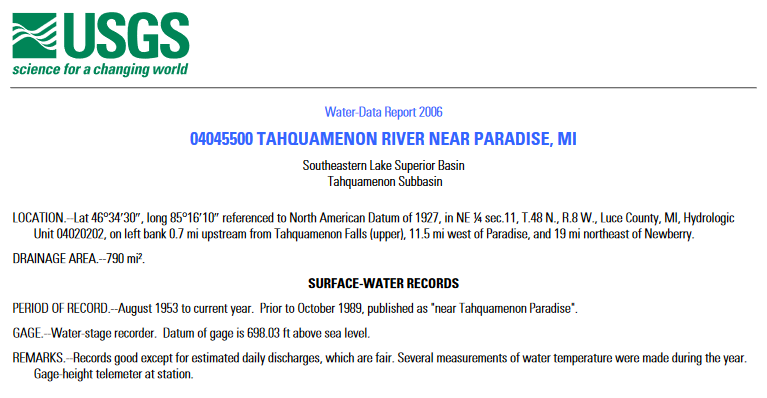
\includegraphics{2006_WaterYearSummaryRemarks.PNG} \\

\textbf{2017 Remarks:}

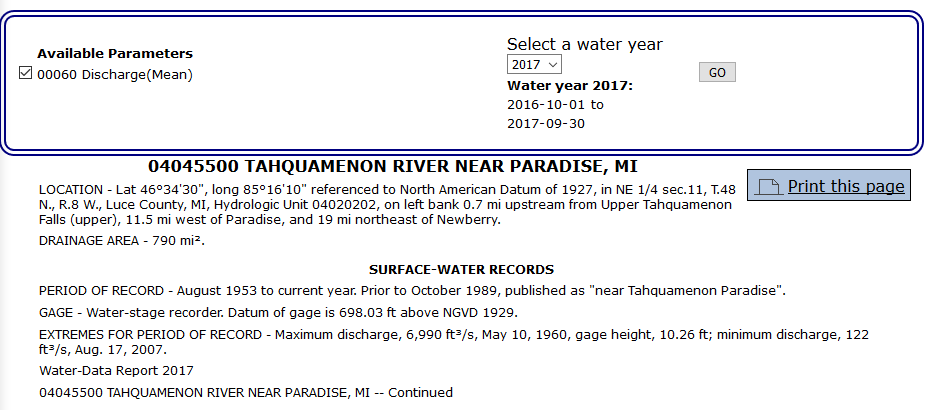
\includegraphics{2017_WaterYearSummaryRemarks.PNG} \\

    \textbf{Part B) Create a table showing the average monthly discharge for
1981 to 2010. Find the 30-year average for your table.}

    \begin{Verbatim}[commandchars=\\\{\}]
{\color{incolor}In [{\color{incolor}89}]:} \PY{k+kn}{import} \PY{n+nn}{pandas} \PY{k}{as} \PY{n+nn}{pd}
         \PY{k+kn}{import} \PY{n+nn}{numpy} \PY{k}{as} \PY{n+nn}{np}
         \PY{k+kn}{import} \PY{n+nn}{datetime} \PY{k}{as} \PY{n+nn}{dt}
         \PY{k+kn}{import} \PY{n+nn}{matplotlib}\PY{n+nn}{.}\PY{n+nn}{pyplot} \PY{k}{as} \PY{n+nn}{plt}
\end{Verbatim}


    \begin{Verbatim}[commandchars=\\\{\}]
{\color{incolor}In [{\color{incolor}112}]:} \PY{n}{Area\PYZus{}mi2} \PY{o}{=} \PY{l+m+mi}{790}
          \PY{n}{Area\PYZus{}ft2} \PY{o}{=} \PY{n}{Area\PYZus{}mi2} \PY{o}{*} \PY{l+m+mi}{27878000}
          \PY{n}{date\PYZus{}range} \PY{o}{=} \PY{p}{(}
              \PY{n}{dt}\PY{o}{.}\PY{n}{datetime}\PY{p}{(}\PY{n}{year}\PY{o}{=}\PY{l+m+mi}{1980}\PY{p}{,}\PY{n}{month}\PY{o}{=}\PY{l+m+mi}{12}\PY{p}{,}\PY{n}{day}\PY{o}{=}\PY{l+m+mi}{29}\PY{p}{)}\PY{p}{,} 
              \PY{n}{dt}\PY{o}{.}\PY{n}{datetime}\PY{p}{(}\PY{n}{year}\PY{o}{=}\PY{l+m+mi}{2010}\PY{p}{,}\PY{n}{month}\PY{o}{=}\PY{l+m+mi}{12}\PY{p}{,}\PY{n}{day}\PY{o}{=}\PY{l+m+mi}{29}\PY{p}{)}
          \PY{p}{)}
\end{Verbatim}


    \begin{Verbatim}[commandchars=\\\{\}]
{\color{incolor}In [{\color{incolor}76}]:} \PY{n}{data} \PY{o}{=} \PY{n}{pd}\PY{o}{.}\PY{n}{read\PYZus{}csv}\PY{p}{(}
             \PY{l+s+s1}{\PYZsq{}}\PY{l+s+s1}{TahquamenonRiver\PYZus{}04045500\PYZus{}MonthlyStatistics.txt}\PY{l+s+s1}{\PYZsq{}}\PY{p}{,}
             \PY{n}{sep} \PY{o}{=} \PY{l+s+s1}{\PYZsq{}}\PY{l+s+se}{\PYZbs{}t}\PY{l+s+s1}{\PYZsq{}}\PY{p}{,}
             \PY{n}{names} \PY{o}{=} \PY{p}{[}\PY{l+s+s1}{\PYZsq{}}\PY{l+s+s1}{Agency}\PY{l+s+s1}{\PYZsq{}}\PY{p}{,}\PY{l+s+s1}{\PYZsq{}}\PY{l+s+s1}{Site Number}\PY{l+s+s1}{\PYZsq{}}\PY{p}{,}\PY{l+s+s1}{\PYZsq{}}\PY{l+s+s1}{Parameter Code}\PY{l+s+s1}{\PYZsq{}}\PY{p}{,}\PY{l+s+s1}{\PYZsq{}}\PY{l+s+s1}{Timeseries ID}\PY{l+s+s1}{\PYZsq{}}\PY{p}{,}
                      \PY{l+s+s1}{\PYZsq{}}\PY{l+s+s1}{Year}\PY{l+s+s1}{\PYZsq{}}\PY{p}{,}\PY{l+s+s1}{\PYZsq{}}\PY{l+s+s1}{Month}\PY{l+s+s1}{\PYZsq{}}\PY{p}{,}\PY{l+s+s1}{\PYZsq{}}\PY{l+s+s1}{Mean Value [ cfs ]}\PY{l+s+s1}{\PYZsq{}}\PY{p}{]}\PY{p}{,}
             \PY{n}{skiprows} \PY{o}{=} \PY{l+m+mi}{37}\PY{p}{,}
             \PY{n}{usecols} \PY{o}{=} \PY{p}{[}\PY{l+m+mi}{4}\PY{p}{,}\PY{l+m+mi}{5}\PY{p}{,}\PY{l+m+mi}{6}\PY{p}{]}
         \PY{p}{)}
         
         \PY{c+c1}{\PYZsh{} Set Years and Months to Type String}
         \PY{n}{data}\PY{o}{.}\PY{n}{Year} \PY{o}{=} \PY{n}{data}\PY{o}{.}\PY{n}{Year}\PY{o}{.}\PY{n}{astype}\PY{p}{(}\PY{n+nb}{str}\PY{p}{)}
         \PY{n}{data}\PY{o}{.}\PY{n}{Month} \PY{o}{=} \PY{n}{data}\PY{o}{.}\PY{n}{Month}\PY{o}{.}\PY{n}{astype}\PY{p}{(}\PY{n+nb}{str}\PY{p}{)}
         
         \PY{c+c1}{\PYZsh{} Join the strings with a \PYZhy{}01\PYZhy{} for the day.}
         \PY{n}{a} \PY{o}{=} \PY{n}{data}\PY{o}{.}\PY{n}{Month} \PY{o}{+} \PY{l+s+s1}{\PYZsq{}}\PY{l+s+s1}{\PYZhy{}01\PYZhy{}}\PY{l+s+s1}{\PYZsq{}}\PY{o}{+} \PY{n}{data}\PY{o}{.}\PY{n}{Year}
         
         \PY{c+c1}{\PYZsh{} Convert to a datatime format}
         \PY{n}{data}\PY{p}{[}\PY{l+s+s1}{\PYZsq{}}\PY{l+s+s1}{Date}\PY{l+s+s1}{\PYZsq{}}\PY{p}{]} \PY{o}{=} \PY{n}{pd}\PY{o}{.}\PY{n}{to\PYZus{}datetime}\PY{p}{(}\PY{n}{a}\PY{p}{)}
         
         \PY{c+c1}{\PYZsh{} Add column for days in the month... includes leap years for February}
         \PY{n}{data}\PY{p}{[}\PY{l+s+s1}{\PYZsq{}}\PY{l+s+s1}{DaysInMonth}\PY{l+s+s1}{\PYZsq{}}\PY{p}{]} \PY{o}{=} \PY{n}{data}\PY{o}{.}\PY{n}{Date}\PY{o}{.}\PY{n}{dt}\PY{o}{.}\PY{n}{daysinmonth}
         
         \PY{c+c1}{\PYZsh{} Revert Month \PYZam{} Year back to type int}
         \PY{n}{data}\PY{o}{.}\PY{n}{Year} \PY{o}{=} \PY{n}{data}\PY{o}{.}\PY{n}{Year}\PY{o}{.}\PY{n}{astype}\PY{p}{(}\PY{n+nb}{str}\PY{p}{)}
         \PY{n}{data}\PY{o}{.}\PY{n}{Month} \PY{o}{=} \PY{n}{data}\PY{o}{.}\PY{n}{Month}\PY{o}{.}\PY{n}{astype}\PY{p}{(}\PY{n+nb}{str}\PY{p}{)}
         
         \PY{c+c1}{\PYZsh{} Select for data in Normal Range}
         \PY{n}{Data\PYZus{}Normal} \PY{o}{=} \PY{n}{data}\PY{p}{[}\PY{n}{data}\PY{p}{[}\PY{l+s+s1}{\PYZsq{}}\PY{l+s+s1}{Date}\PY{l+s+s1}{\PYZsq{}}\PY{p}{]}\PY{o}{\PYZgt{}}\PY{n}{date\PYZus{}range}\PY{p}{[}\PY{l+m+mi}{0}\PY{p}{]}\PY{p}{]}
         \PY{n}{Data\PYZus{}Normal} \PY{o}{=}  \PY{n}{Data\PYZus{}Normal}\PY{p}{[}\PY{n}{Data\PYZus{}Normal}\PY{p}{[}\PY{l+s+s1}{\PYZsq{}}\PY{l+s+s1}{Date}\PY{l+s+s1}{\PYZsq{}}\PY{p}{]}\PY{o}{\PYZlt{}}\PY{n}{date\PYZus{}range}\PY{p}{[}\PY{l+m+mi}{1}\PY{p}{]}\PY{p}{]}
\end{Verbatim}



\textbf{CFS to Total Volume}

Have flow in \(\frac{ft^3}{s}\), want \(\frac{ft^3}{month}\).

To accomplish do the following:
\[\frac{ft^3}{s} * \frac{60 s}{1 min} * \frac{60 min}{1 hr} * \frac{24 hr}{1 day} * \frac{Days In Month}{1 month} = \big[\frac{ft^3}{month}\big] \]

    \begin{Verbatim}[commandchars=\\\{\}]
{\color{incolor}In [{\color{incolor}107}]:} \PY{c+c1}{\PYZsh{} Compute Monthly Discharges in Cubic Feet}
          \PY{n}{Data\PYZus{}Normal}\PY{p}{[}\PY{l+s+s1}{\PYZsq{}}\PY{l+s+s1}{Volume\PYZus{}ft3}\PY{l+s+s1}{\PYZsq{}}\PY{p}{]} \PY{o}{=} \PY{n}{Data\PYZus{}Normal}\PY{p}{[}\PY{l+s+s1}{\PYZsq{}}\PY{l+s+s1}{Mean Value [ cfs ]}\PY{l+s+s1}{\PYZsq{}}\PY{p}{]} \PYZbs{}
              \PY{o}{*} \PY{n}{Data\PYZus{}Normal}\PY{p}{[}\PY{l+s+s1}{\PYZsq{}}\PY{l+s+s1}{DaysInMonth}\PY{l+s+s1}{\PYZsq{}}\PY{p}{]} \PY{o}{*} \PY{l+m+mi}{60} \PY{o}{*} \PY{l+m+mi}{60} \PY{o}{*} \PY{l+m+mi}{24}
\end{Verbatim}


    \textbf{Total Volume to Depth in Inches}

To calculate this volume in inches on the watershed:

\[ \frac{ft^3}{month} * \frac{1}{Watershed Area} * \frac{12 in}{1 ft} = \big[\frac{in}{month}\big] \]

    \begin{Verbatim}[commandchars=\\\{\}]
{\color{incolor}In [{\color{incolor}78}]:} \PY{c+c1}{\PYZsh{} Compute Monthly Discharge in Inches}
         \PY{n}{Data\PYZus{}Normal}\PY{p}{[}\PY{l+s+s1}{\PYZsq{}}\PY{l+s+s1}{Volume [ in ]}\PY{l+s+s1}{\PYZsq{}}\PY{p}{]} \PY{o}{=} \PY{n}{Data\PYZus{}Normal}\PY{p}{[}\PY{l+s+s1}{\PYZsq{}}\PY{l+s+s1}{Volume\PYZus{}ft3}\PY{l+s+s1}{\PYZsq{}}\PY{p}{]} \PY{o}{/} \PY{n}{Area\PYZus{}ft2} \PY{o}{*} \PY{l+m+mi}{12}
\end{Verbatim}


    \textbf{Prepare Table}

    \begin{Verbatim}[commandchars=\\\{\}]
{\color{incolor}In [{\color{incolor}109}]:} \PY{n}{Months} \PY{o}{=} \PY{n}{Data\PYZus{}Normal}\PY{o}{.}\PY{n}{drop}\PY{p}{(}\PY{n}{columns}\PY{o}{=}\PY{p}{[}\PY{l+s+s1}{\PYZsq{}}\PY{l+s+s1}{DaysInMonth}\PY{l+s+s1}{\PYZsq{}}\PY{p}{,}\PY{l+s+s1}{\PYZsq{}}\PY{l+s+s1}{Volume\PYZus{}ft3}\PY{l+s+s1}{\PYZsq{}}\PY{p}{]}\PY{p}{)}\PY{o}{.}\PY{n}{groupby}\PY{p}{(}\PY{l+s+s1}{\PYZsq{}}\PY{l+s+s1}{Month}\PY{l+s+s1}{\PYZsq{}}\PY{p}{)}
          \PY{n}{Months} \PY{o}{=} \PY{n}{Months}\PY{o}{.}\PY{n}{mean}\PY{p}{(}\PY{p}{)}
          
          \PY{c+c1}{\PYZsh{} Need to reorder the table by month now}
          \PY{n}{Month\PYZus{}str} \PY{o}{=} \PY{n}{Months}\PY{o}{.}\PY{n}{reindex}\PY{p}{(}
              \PY{n}{index}\PY{o}{=}\PY{p}{[}\PY{l+s+s1}{\PYZsq{}}\PY{l+s+s1}{January}\PY{l+s+s1}{\PYZsq{}}\PY{p}{,}\PY{l+s+s1}{\PYZsq{}}\PY{l+s+s1}{October}\PY{l+s+s1}{\PYZsq{}}\PY{p}{,}\PY{l+s+s1}{\PYZsq{}}\PY{l+s+s1}{November}\PY{l+s+s1}{\PYZsq{}}\PY{p}{,}\PY{l+s+s1}{\PYZsq{}}\PY{l+s+s1}{December}\PY{l+s+s1}{\PYZsq{}}\PY{p}{,}
                     \PY{l+s+s1}{\PYZsq{}}\PY{l+s+s1}{February}\PY{l+s+s1}{\PYZsq{}}\PY{p}{,}\PY{l+s+s1}{\PYZsq{}}\PY{l+s+s1}{March}\PY{l+s+s1}{\PYZsq{}}\PY{p}{,}\PY{l+s+s1}{\PYZsq{}}\PY{l+s+s1}{April}\PY{l+s+s1}{\PYZsq{}}\PY{p}{,}\PY{l+s+s1}{\PYZsq{}}\PY{l+s+s1}{May}\PY{l+s+s1}{\PYZsq{}}\PY{p}{,}
                     \PY{l+s+s1}{\PYZsq{}}\PY{l+s+s1}{June}\PY{l+s+s1}{\PYZsq{}}\PY{p}{,}\PY{l+s+s1}{\PYZsq{}}\PY{l+s+s1}{July}\PY{l+s+s1}{\PYZsq{}}\PY{p}{,}\PY{l+s+s1}{\PYZsq{}}\PY{l+s+s1}{August}\PY{l+s+s1}{\PYZsq{}}\PY{p}{,}\PY{l+s+s1}{\PYZsq{}}\PY{l+s+s1}{September}\PY{l+s+s1}{\PYZsq{}}\PY{p}{]}
          \PY{p}{)}
          \PY{k}{for} \PY{n}{i} \PY{o+ow}{in} \PY{n+nb}{range}\PY{p}{(}\PY{l+m+mi}{0}\PY{p}{,}\PY{l+m+mi}{12}\PY{p}{)}\PY{p}{:}
              \PY{n}{Month\PYZus{}str}\PY{o}{.}\PY{n}{iloc}\PY{p}{[}\PY{n}{i}\PY{p}{]} \PY{o}{=} \PY{n}{Months}\PY{o}{.}\PY{n}{iloc}\PY{p}{[}\PY{n}{i}\PY{p}{]}
          \PY{n}{Month\PYZus{}str} \PY{o}{=} \PY{n}{Month\PYZus{}str}\PY{o}{.}\PY{n}{reindex}\PY{p}{(}
              \PY{p}{[}\PY{l+s+s1}{\PYZsq{}}\PY{l+s+s1}{January}\PY{l+s+s1}{\PYZsq{}}\PY{p}{,}\PY{l+s+s1}{\PYZsq{}}\PY{l+s+s1}{February}\PY{l+s+s1}{\PYZsq{}}\PY{p}{,}\PY{l+s+s1}{\PYZsq{}}\PY{l+s+s1}{March}\PY{l+s+s1}{\PYZsq{}}\PY{p}{,}\PY{l+s+s1}{\PYZsq{}}\PY{l+s+s1}{April}\PY{l+s+s1}{\PYZsq{}}\PY{p}{,}
               \PY{l+s+s1}{\PYZsq{}}\PY{l+s+s1}{May}\PY{l+s+s1}{\PYZsq{}}\PY{p}{,}\PY{l+s+s1}{\PYZsq{}}\PY{l+s+s1}{June}\PY{l+s+s1}{\PYZsq{}}\PY{p}{,}\PY{l+s+s1}{\PYZsq{}}\PY{l+s+s1}{July}\PY{l+s+s1}{\PYZsq{}}\PY{p}{,}\PY{l+s+s1}{\PYZsq{}}\PY{l+s+s1}{August}\PY{l+s+s1}{\PYZsq{}}\PY{p}{,}
               \PY{l+s+s1}{\PYZsq{}}\PY{l+s+s1}{September}\PY{l+s+s1}{\PYZsq{}}\PY{p}{,}\PY{l+s+s1}{\PYZsq{}}\PY{l+s+s1}{October}\PY{l+s+s1}{\PYZsq{}}\PY{p}{,}\PY{l+s+s1}{\PYZsq{}}\PY{l+s+s1}{November}\PY{l+s+s1}{\PYZsq{}}\PY{p}{,}\PY{l+s+s1}{\PYZsq{}}\PY{l+s+s1}{December}\PY{l+s+s1}{\PYZsq{}}\PY{p}{]}
          \PY{p}{)}
          \PY{n}{Month\PYZus{}str}
\end{Verbatim}


\begin{Verbatim}[commandchars=\\\{\}]
{\color{outcolor}Out[{\color{outcolor}109}]:}            Mean Value [ cfs ]  Volume [ in ]
          Month                                       
          January            548.5       0.80
          February           495.5       0.66
          March              855.5       1.26
          April             2636.5       3.72
          May               1251.0       1.83
          June               579.5       0.82
          July               420.0       0.61
          August             377.3       0.55
          September          494.4       0.70
          October            859.1       1.25
          November           992.8       1.40
          December           783.8       1.14
\end{Verbatim}
            
    \textbf{Part C) Create a table showing the average monthly precipitation
(in inches) for the watershed.} \\

\href{https://www.ncdc.noaa.gov/cdo-web/datasets/NORMAL_DLY/stations/GHCND:USC00208043/detail}{Tahquamenon
Falls State Park Weather Station (USC00208042)} is located approximately
3 miles from the USGS stream gage. The 1981-2010 Precipitation normals
in inches for each month are located below.

    \begin{Verbatim}[commandchars=\\\{\}]
{\color{incolor}In [{\color{incolor}113}]:} \PY{n}{months} \PY{o}{=} \PY{p}{[}
              \PY{l+s+s1}{\PYZsq{}}\PY{l+s+s1}{January}\PY{l+s+s1}{\PYZsq{}}\PY{p}{,}\PY{l+s+s1}{\PYZsq{}}\PY{l+s+s1}{February}\PY{l+s+s1}{\PYZsq{}}\PY{p}{,}\PY{l+s+s1}{\PYZsq{}}\PY{l+s+s1}{March}\PY{l+s+s1}{\PYZsq{}}\PY{p}{,}\PY{l+s+s1}{\PYZsq{}}\PY{l+s+s1}{April}\PY{l+s+s1}{\PYZsq{}}\PY{p}{,}
              \PY{l+s+s1}{\PYZsq{}}\PY{l+s+s1}{May}\PY{l+s+s1}{\PYZsq{}}\PY{p}{,}\PY{l+s+s1}{\PYZsq{}}\PY{l+s+s1}{June}\PY{l+s+s1}{\PYZsq{}}\PY{p}{,}\PY{l+s+s1}{\PYZsq{}}\PY{l+s+s1}{July}\PY{l+s+s1}{\PYZsq{}}\PY{p}{,}\PY{l+s+s1}{\PYZsq{}}\PY{l+s+s1}{August}\PY{l+s+s1}{\PYZsq{}}\PY{p}{,}
              \PY{l+s+s1}{\PYZsq{}}\PY{l+s+s1}{September}\PY{l+s+s1}{\PYZsq{}}\PY{p}{,}\PY{l+s+s1}{\PYZsq{}}\PY{l+s+s1}{October}\PY{l+s+s1}{\PYZsq{}}\PY{p}{,}\PY{l+s+s1}{\PYZsq{}}\PY{l+s+s1}{November}\PY{l+s+s1}{\PYZsq{}}\PY{p}{,}\PY{l+s+s1}{\PYZsq{}}\PY{l+s+s1}{December}\PY{l+s+s1}{\PYZsq{}}
          \PY{p}{]}
          \PY{n}{precip} \PY{o}{=} \PY{p}{[}
              \PY{l+m+mf}{3.12}\PY{p}{,} \PY{l+m+mf}{1.91}\PY{p}{,} \PY{l+m+mf}{2.16}\PY{p}{,} \PY{l+m+mf}{2.34}\PY{p}{,}
              \PY{l+m+mf}{2.74}\PY{p}{,} \PY{l+m+mf}{2.93}\PY{p}{,} \PY{l+m+mf}{3.04}\PY{p}{,} \PY{l+m+mf}{3.41}\PY{p}{,} 
              \PY{l+m+mf}{3.72}\PY{p}{,} \PY{l+m+mf}{4.10}\PY{p}{,} \PY{l+m+mf}{3.27}\PY{p}{,} \PY{l+m+mf}{3.44}
          \PY{p}{]}
          
          \PY{n}{Precip\PYZus{}Normal} \PY{o}{=} \PY{n+nb}{dict}\PY{p}{(}\PY{n+nb}{zip}\PY{p}{(}\PY{n}{months}\PY{p}{,}\PY{n}{precip}\PY{p}{)}\PY{p}{)}
          \PY{n}{Precip\PYZus{}Normal} \PY{o}{=} \PY{n}{pd}\PY{o}{.}\PY{n}{DataFrame}\PY{o}{.}\PY{n}{from\PYZus{}dict}\PY{p}{(}\PY{n}{Precip\PYZus{}Normal}\PY{p}{,} \PY{n}{orient}\PY{o}{=}\PY{l+s+s1}{\PYZsq{}}\PY{l+s+s1}{index}\PY{l+s+s1}{\PYZsq{}}\PY{p}{,} \PY{p}{)}
          \PY{n}{Precip\PYZus{}Normal} \PY{o}{=} \PY{n}{Precip\PYZus{}Normal}\PY{o}{.}\PY{n}{rename}\PY{p}{(}
              \PY{n}{index}\PY{o}{=}\PY{n+nb}{str}\PY{p}{,} 
              \PY{n}{columns}\PY{o}{=}\PY{p}{\PYZob{}}\PY{l+m+mi}{0}\PY{p}{:}\PY{l+s+s1}{\PYZsq{}}\PY{l+s+s1}{Precip Normals [ in ]}\PY{l+s+s1}{\PYZsq{}}\PY{p}{\PYZcb{}}
          \PY{p}{)}
          \PY{n}{Precip\PYZus{}Normal}
\end{Verbatim}

\pagebreak
\begin{Verbatim}[commandchars=\\\{\}]
{\color{outcolor}Out[{\color{outcolor}113}]:}            Precip Normals [ in ]
          January                     3.12
          February                    1.91
          March                       2.16
          April                       2.34
          May                         2.74
          June                        2.93
          July                        3.04
          August                      3.41
          September                   3.72
          October                     4.10
          November                    3.27
          December                    3.44
\end{Verbatim}
            
     \textbf{Part D) Plot the average monthly precipitation (in inches) and
the average monthly discharge (in inches) versus month.} \\

    \begin{Verbatim}[commandchars=\\\{\}]
{\color{incolor}In [{\color{incolor}117}]:} \PY{n}{fig}\PY{p}{,} \PY{n}{ax} \PY{o}{=} \PY{n}{plt}\PY{o}{.}\PY{n}{subplots}\PY{p}{(}\PY{n}{figsize}\PY{o}{=}\PY{p}{(}\PY{l+m+mi}{10}\PY{p}{,}\PY{l+m+mi}{10}\PY{p}{)}\PY{p}{)}
          
          \PY{n}{Precip\PYZus{}Normal}\PY{o}{.}\PY{n}{plot}\PY{p}{(}\PY{n}{ax}\PY{o}{=}\PY{n}{ax}\PY{p}{,}\PY{n}{xticks}\PY{o}{=}\PY{n}{np}\PY{o}{.}\PY{n}{arange}\PY{p}{(}\PY{l+m+mi}{12}\PY{p}{)}\PY{p}{,}\PY{n}{legend}\PY{o}{=}\PY{k+kc}{True}\PY{p}{)}
          \PY{n}{Month\PYZus{}str}\PY{p}{[}\PY{l+s+s1}{\PYZsq{}}\PY{l+s+s1}{Volume [ in ]}\PY{l+s+s1}{\PYZsq{}}\PY{p}{]}\PY{o}{.}\PY{n}{plot}\PY{p}{(}\PY{n}{ax}\PY{o}{=}\PY{n}{ax}\PY{p}{,}\PY{n}{xticks}\PY{o}{=}\PY{n}{np}\PY{o}{.}\PY{n}{arange}\PY{p}{(}\PY{l+m+mi}{12}\PY{p}{)}\PY{p}{,}\PY{n}{legend}\PY{o}{=}\PY{k+kc}{True}\PY{p}{)}
          
          \PY{n}{plt}\PY{o}{.}\PY{n}{xticks}\PY{p}{(}\PY{n}{rotation}\PY{o}{=}\PY{l+s+s1}{\PYZsq{}}\PY{l+s+s1}{vertical}\PY{l+s+s1}{\PYZsq{}}\PY{p}{)}
          \PY{n}{plt}\PY{o}{.}\PY{n}{ylabel}\PY{p}{(}\PY{l+s+s1}{\PYZsq{}}\PY{l+s+s1}{Depth [in]}\PY{l+s+s1}{\PYZsq{}}\PY{p}{)}
          \PY{n}{plt}\PY{o}{.}\PY{n}{xlabel}\PY{p}{(}\PY{l+s+s1}{\PYZsq{}}\PY{l+s+s1}{Month}\PY{l+s+s1}{\PYZsq{}}\PY{p}{)}
          \PY{n}{plt}\PY{o}{.}\PY{n}{title}\PY{p}{(}
              \PY{l+s+s1}{\PYZsq{}}\PY{l+s+s1}{Average Precipitation and Volume Discharge for Tahquemenon River}\PY{l+s+se}{\PYZbs{}}
          \PY{l+s+s1}{ Watershed, 1980\PYZhy{}2010}\PY{l+s+s1}{\PYZsq{}}
          \PY{p}{)}
          \PY{n}{plt}\PY{o}{.}\PY{n}{show}\PY{p}{(}\PY{p}{)}
\end{Verbatim}


    \begin{center}
    \adjustimage{max size={0.9\linewidth}{0.9\paperheight}}{output_14_0.png}
    \end{center}
    { \hspace*{\fill} \\}
    
     \textbf{Part E) Compute the average annual precipitation (in inches).} \\

From the Tahquemon Falls State Park Station report, \textbf{annual
precipitation is 36.18 inches}. This is confirmed when taking the sum of
the monthly averages.\\

     \textbf{Part F) Compute the average annual discharge (in inches).}\\

Below is a table of the total volume discharge per year. Taking the
average of this table, we find that the \textbf{average annual discharge
is 14.74 inches.}\\

    \begin{Verbatim}[commandchars=\\\{\}]
{\color{incolor}In [{\color{incolor}99}]:} \PY{n}{Year} \PY{o}{=} \PY{n}{Data\PYZus{}Normal}\PY{o}{.}\PY{n}{drop}\PY{p}{(}\PY{n}{columns}\PY{o}{=}\PY{p}{[}\PY{l+s+s1}{\PYZsq{}}\PY{l+s+s1}{DaysInMonth}\PY{l+s+s1}{\PYZsq{}}\PY{p}{,}\PY{l+s+s1}{\PYZsq{}}\PY{l+s+s1}{Volume\PYZus{}ft3}\PY{l+s+s1}{\PYZsq{}}\PY{p}{]}\PY{p}{)}\PY{o}{.}\PY{n}{groupby}\PY{p}{(}\PY{l+s+s1}{\PYZsq{}}\PY{l+s+s1}{Year}\PY{l+s+s1}{\PYZsq{}}\PY{p}{)}
         \PY{n}{Year}\PY{o}{.}\PY{n}{sum}\PY{p}{(}\PY{p}{)}
\end{Verbatim}


\begin{Verbatim}[commandchars=\\\{\}]
{\color{outcolor}Out[{\color{outcolor}99}]:}       Mean Value [ cfs ]  Volume [ in ]
         Year                                   
         1981             10196.6      14.57
         1982             13152.0      18.86
         1983             10354.7      14.85
         1984             11219.5      16.05
         1985             12486.7      17.88
         1986              9667.7      13.79
         1987              8357.6      11.99
         1988             11649.8      16.65
         1989              8904.8      12.71
         1990             11330.1      16.25
         1991              9893.3      14.14
         1992             10411.8      14.94
         1993             12254.2      17.56
         1994              9527.6      13.64
         1995              9691.4      13.90
         1996             13820.0      19.87
         1997             10017.1      14.32
         1998              7512.9      10.70
         1999              8631.1      12.29
         2000              6980.8      10.04
         2001             12527.3      17.95
         2002             12118.5      17.36
         2003              9728.4      13.91
         2004             11810.8      16.92
         2005              8804.2      12.57
         2006              8881.9      12.71
         2007              8515.1      12.19
         2008             11128.1      15.94
         2009             10017.8      14.35
         2010              9222.6      13.21
\end{Verbatim}
            
    \begin{Verbatim}[commandchars=\\\{\}]
{\color{incolor}In [{\color{incolor}87}]:} \PY{n}{Year}\PY{o}{.}\PY{n}{sum}\PY{p}{(}\PY{p}{)}\PY{o}{.}\PY{n}{mean}\PY{p}{(}\PY{p}{)}
\end{Verbatim}


\begin{Verbatim}[commandchars=\\\{\}]
{\color{outcolor}Out[{\color{outcolor}87}]:} Mean Value [ cfs ]    10293.8
         Volume [ in ]            14.74
         dtype: float64
\end{Verbatim}
 

     \textbf{Part G) Compute the average annual evapotranspiration (in
inches) using the long-term water budget assumption.}\\

The long-term water budget assumption is that precipitation is equal to
the sum of the basin's evapotranspiration and the surface (river)
discharge, or \[P = E + Q_{0}\]

Solving for our evapotranspiration term, \(E\): \[E = P - Q_{0}\]

Plugging in our numbers to this equation we find that:

\[E = 36.18 - 14.74\]

\[E = 21.44 inches\]

     \textbf{Part H) Compute the runoff coefficient (i.e., annual discharge
as a fraction of precipitation), in percent.}\\

\[C_{runoff} = \frac{Depth_{discharge}}{Depth_{precipitation}}*100\%\]

\[C_{runoff} = \frac{14.74}{36.18} * 100 \%\]

\[C_{runoff} = 41.74 \%\]

Considering that this watershed is almost completely forested in a
national forest and state park, it makes sense that the number would be
lower.\\

    \textbf{Note: Streamstats isn't available in Michigan.}


    % Add a bibliography block to the postdoc
    
    
    
    \end{document}
